\documentclass[11pt]{article}
\usepackage[notes]{la}
\lamodule{1}{9}{The Matrix of a Linear Transformation}
\laxdoc{1.4}
\laxdoc{1.5}
\laxdoc{1.7}
\laxdoc{1.8}

\begin{document}

\section{The Matrix of a Linear Transformation}

\begin{guide}
In Section~1.8 every matrix gave a linear transformation. Now turn the question around. Suppose someone hands you a linear transformation as a \emph{rule}: ``rotate the plane by $30^\circ$'', or ``reflect in a line'', or a formula. Is it always given by a matrix? If so, which matrix, and how do you find it quickly, ideally by looking at a picture? And once you have the matrix, what do the pivots say about whether the map is one-to-one or onto?
\end{guide}

\textbf{By the end of this section you should be able to:}
\begin{itemize}
  \item state and prove that every linear transformation $\R^n\to\R^m$ is a matrix transformation, and name its \emph{standard matrix};
  \item find the standard matrix from a formula, from the images of $\bv{e}_1,\dots,\bv{e}_n$, from other known values, or from a picture;
  \item write down the matrices of rotations, reflections, shears, stretches and projections of the plane and read their geometric effect from the columns;
  \item find the matrix of ``do this, then that'' by following $\bv{e}_1$ and $\bv{e}_2$ through both steps, and explain why the order matters;
  \item define \emph{one-to-one} and \emph{onto} and decide each from the pivots of the standard matrix;
  \item explain, with a picture, why a map from $\R^2$ to $\R^3$ cannot be onto and a map from $\R^3$ to $\R^2$ cannot be one-to-one;
  \item connect a flattening map (a projection) with the area of the image of the unit square.
\end{itemize}

% ---------------------------------------------------------------------
\subsection*{Every linear map is a matrix map}

Let $T:\R^2\to\R^2$ be linear, and suppose all we know is where the two standard unit vectors go: $T(\bv{e}_1)=(1,3)$ and $T(\bv{e}_2)=(-2,4)$. What is $T(5,-1)$? Write $(5,-1)=5\bv{e}_1-\bv{e}_2$ and use superposition (Theorem~\ref{1.8-thm:props}):
\[
T(5,-1)=5\,T(\bv{e}_1)-T(\bv{e}_2)=5\begin{bmatrix}1\\3\end{bmatrix}-\begin{bmatrix}-2\\4\end{bmatrix}=\begin{bmatrix}7\\11\end{bmatrix}.
\]
This is the same arithmetic as a matrix--vector product, with $T(\bv{e}_1)$ and $T(\bv{e}_2)$ as the columns. We now show that this is always the case.

\begin{defn}{Standard matrix}{stdmat}
Let $T:\R^n\to\R^m$ be a linear transformation. The \emph{standard matrix} of $T$ is the $m\times n$ matrix
\[
A=\begin{bmatrix}T(\bv{e}_1)&T(\bv{e}_2)&\cdots&T(\bv{e}_n)\end{bmatrix},
\]
whose $j$th column is the image of the $j$th standard unit vector $\bv{e}_j$ (Example~\ref{1.4-ex:ei}).
\end{defn}

\begin{thm}{Linear maps are matrix maps}{stdthm}
Let $T:\R^n\to\R^m$ be a linear transformation. Then there is a \emph{unique} matrix $A$ such that $T(\bv{x})=A\bv{x}$ for all $\bv{x}$ in $\R^n$, namely the standard matrix of $T$.
\end{thm}

\begin{proof}
Every $\bv{x}=(x_1,\dots,x_n)$ is the combination $\bv{x}=x_1\bv{e}_1+\cdots+x_n\bv{e}_n$. By superposition (Theorem~\ref{1.8-thm:props}(c)),
\[
T(\bv{x})=x_1T(\bv{e}_1)+\cdots+x_nT(\bv{e}_n)=\begin{bmatrix}T(\bv{e}_1)&\cdots&T(\bv{e}_n)\end{bmatrix}\begin{bmatrix}x_1\\\vdots\\x_n\end{bmatrix}=A\bv{x}.
\]
For uniqueness, suppose $T(\bv{x})=B\bv{x}$ for every $\bv{x}$. Then $\bv{b}_j=B\bv{e}_j=T(\bv{e}_j)$ is the $j$th column of $A$, so $B=A$.
\end{proof}

Theorem~\ref{thm:stdthm} together with Theorem~\ref{1.8-thm:matlin} says that \emph{linear transformation} and \emph{matrix transformation} are two names for one thing. It also says that $m\times n$ matrices and linear maps $\R^n\to\R^m$ correspond exactly. In the plane the picture is this: the columns of $A$ are where $\bv{e}_1$ and $\bv{e}_2$ land, and everything else follows by the parallelogram rule.

\begin{center}
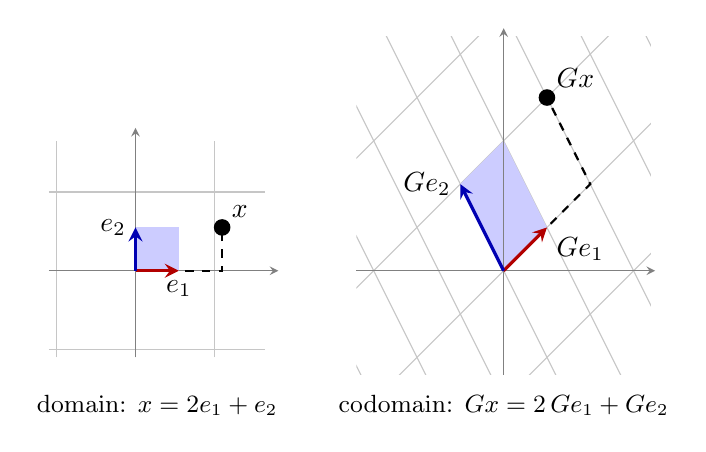
\begin{tikzpicture}[x=0.55cm,y=0.55cm,>=stealth]
  \draw[gray!45] (-2,-2) grid (3,3);
  \draw[->,gray] (-2,0)--(3.3,0); \draw[->,gray] (0,-2)--(0,3.3);
  \fill[blue!20] (0,0) rectangle (1,1);
  \draw[dashed,thick] (0,0)--(2,0)--(2,1);
  \draw[->,very thick,red!70!black] (0,0)--(1,0);
  \draw[->,very thick,blue!70!black] (0,0)--(0,1);
  \fill (2,1) circle (3pt);
  \node[below] at (1,0) {$e_1$};
  \node[left] at (0,1) {$e_2$};
  \node[above right] at (2,1) {$x$};
  \node at (0.5,-3.1) {\small domain: $x=2e_1+e_2$};
  \begin{scope}[shift={(8.5,0)}]
    \begin{scope}
      \clip (-3.4,-2.4) rectangle (3.4,5.4);
      \begin{scope}[cm={1,1,-1,2,(0,0)}]
        \foreach \k in {-6,...,6}{\draw[gray!45] (\k,-6)--(\k,6); \draw[gray!45] (-6,\k)--(6,\k);}
        \fill[blue!20] (0,0) rectangle (1,1);
      \end{scope}
    \end{scope}
    \draw[->,gray] (-3.4,0)--(3.5,0); \draw[->,gray] (0,-2.4)--(0,5.6);
    \draw[dashed,thick] (0,0)--(2,2)--(1,4);
    \draw[->,very thick,red!70!black] (0,0)--(1,1);
    \draw[->,very thick,blue!70!black] (0,0)--(-1,2);
    \fill (1,4) circle (3pt);
    \node[below right] at (1,1) {$Ge_1$};
    \node[left] at (-1,2) {$Ge_2$};
    \node[above right] at (1,4) {$Gx$};
    \node at (0,-3.1) {\small codomain: $Gx=2\,Ge_1+Ge_2$};
  \end{scope}
\end{tikzpicture}
\end{center}

\textbf{Figure.} A linear map $G$ with $G\bv{e}_1=(1,1)$ and $G\bv{e}_2=(-1,2)$, so $G=\begin{bmatrix}1&-1\\1&2\end{bmatrix}$. To find $G\bv{x}$ for $\bv{x}=(2,1)$, walk \emph{two} steps along the image of $\bv{e}_1$ and then \emph{one} step along the image of $\bv{e}_2$: the dashed path leads to $G\bv{x}=(1,4)$. The picture of the domain is carried to the picture in the codomain; the grid is re-drawn using the new pair of axes.

\begin{warn}[Columns are not rows]
The images of $\bv{e}_1,\dots,\bv{e}_n$ become the \emph{columns} of $A$, not the rows. A common slip is to write the vectors $T(\bv{e}_1)=(1,3)$ and $T(\bv{e}_2)=(-2,4)$ as rows, which produces the transpose, a different transformation. The check is always: $A\bv{e}_1$ must give back $T(\bv{e}_1)$, because $A\bv{e}_1$ is the first column of $A$.
\end{warn}

\begin{proc}{Finding the standard matrix}{findmat}
\begin{enumerate}
  \item Find the image $T(\bv{e}_j)$ of each standard unit vector $\bv{e}_1,\dots,\bv{e}_n$. (If $T$ is given by a formula, substitute $\bv{e}_j$; if it is given by a picture or description, read off where $\bv{e}_j$ lands; if it is given by values at other vectors, write $\bv{e}_j$ as a combination of those vectors and use superposition, as in Example~\ref{1.8-ex:values}.)
  \item Put $T(\bv{e}_1),\dots,T(\bv{e}_n)$ in the columns of an $m\times n$ matrix.
  \item Check: $A\bv{x}$ should reproduce $T(\bv{x})$ for at least one vector that is not a unit vector.
\end{enumerate}
\end{proc}

\begin{exmp}{From a formula}{formula}
Find the standard matrix of $T(x_1,x_2,x_3)=(x_1-2x_2+x_3,\ 3x_1+x_3)$, from $\R^3$ to $\R^2$.

\textbf{Solution.} Substitute the unit vectors:
\[
T(\bv{e}_1)=T(1,0,0)=(1,3),\qquad T(\bv{e}_2)=T(0,1,0)=(-2,0),\qquad T(\bv{e}_3)=T(0,0,1)=(1,1).
\]
So $A=\begin{bmatrix}1&-2&1\\3&0&1\end{bmatrix}$. Notice that the $j$th column is the list of coefficients of $x_j$ in the formula: reading the formula row by row gives the rows of $A$, which is how you can write the matrix down in one pass. Check with $\bv{x}=(2,1,-1)$: the formula gives $(2-2-1,\ 6-1)=(-1,5)$, and $A\bv{x}=2(1,3)+(-2,0)-(1,1)=(2-2-1,\ 6+0-1)=(-1,5)$. \ $\checkmark$
\end{exmp}

\begin{exmp}{From values at other vectors}{othervals}
Let $T:\R^2\to\R^2$ be linear with $T(1,2)=(3,1)$ and $T(0,1)=(1,-1)$. Find its standard matrix.

\textbf{Solution.} The vector $\bv{e}_2=(0,1)$ is given, so $T(\bv{e}_2)=(1,-1)$. For $\bv{e}_1$ write $(1,0)=(1,2)-2(0,1)$, hence
\[
T(\bv{e}_1)=T(1,2)-2T(0,1)=(3,1)-2(1,-1)=(1,3).
\]
So $A=\begin{bmatrix}1&1\\3&-1\end{bmatrix}$. Check: $A(1,2)=(1+2,\ 3-2)=(3,1)$. \ $\checkmark$
\end{exmp}

\begin{kc}{Matrix from data}{matdata}
(a)~A linear $T:\R^2\to\R^2$ has $T(\bv{e}_1)=(2,-1)$ and $T(\bv{e}_2)=(0,3)$. Write its standard matrix and compute $T(3,-2)$. (b)~Find the standard matrix of $T(x_1,x_2,x_3,x_4)=(x_1+4x_4,\ x_2-x_3)$. What are its dimensions?
\end{kc}

\begin{think}{Why the unit vectors?}{whyunit}
(a)~Could two different matrices define the same linear transformation? Use Theorem~\ref{thm:stdthm}. (b)~In Example~\ref{1.8-ex:values} we found a matrix from the values at $\bv{u}=(1,2)$ and $\bv{v}=(1,3)$ instead of $\bv{e}_1,\bv{e}_2$. In general, if you know $T$ on $n$ vectors $\bv{v}_1,\dots,\bv{v}_n$ of $\R^n$, what must be true of these vectors so that the standard matrix is determined?
\end{think}

% ---------------------------------------------------------------------
\subsection*{Rotations}

Rotate the plane counterclockwise about the origin by an angle $\theta$, and call the result $R_\theta$. Is $R_\theta$ linear? Rotation carries every parallelogram to a congruent parallelogram, so it carries the far corner of the parallelogram on $\bv{u},\bv{v}$ to the far corner of the parallelogram on $R_\theta\bv{u},R_\theta\bv{v}$: $R_\theta(\bv{u}+\bv{v})=R_\theta\bv{u}+R_\theta\bv{v}$. And it does not change lengths, so stretching and then rotating equals rotating and then stretching: $R_\theta(c\bv{u})=cR_\theta\bv{u}$. So $R_\theta$ is linear, and by Theorem~\ref{thm:stdthm} it has a standard matrix; we find it by following $\bv{e}_1$ and $\bv{e}_2$.

\begin{center}
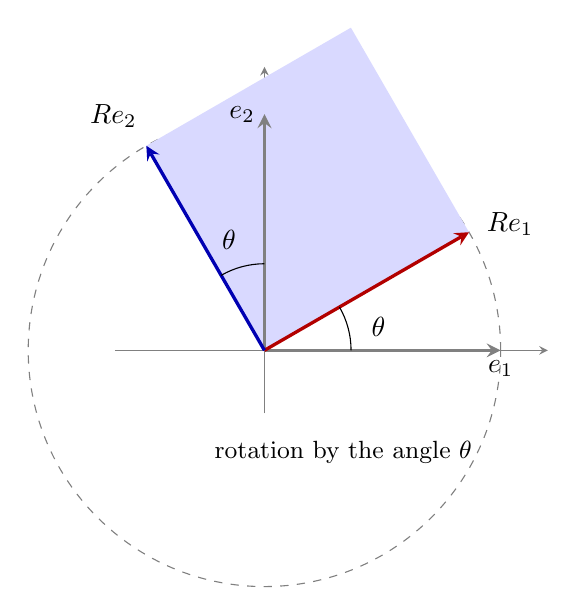
\begin{tikzpicture}[>=stealth]
  \draw[->,gray] (-1.9,0)--(3.6,0); \draw[->,gray] (0,-0.8)--(0,3.6);
  \draw[gray,dashed] (0,0) circle (3);
  \fill[blue!15] (0,0)--(2.598,1.5)--(1.098,4.098)--(-1.5,2.598)--cycle;
  \draw[->,very thick,gray] (0,0)--(3,0);
  \draw[->,very thick,gray] (0,0)--(0,3);
  \draw[->,very thick,red!70!black] (0,0)--(2.598,1.5);
  \draw[->,very thick,blue!70!black] (0,0)--(-1.5,2.598);
  \draw (1.1,0) arc (0:30:1.1);
  \draw (0,1.1) arc (90:120:1.1);
  \node at (1.45,0.3) {$\theta$};
  \node at (-0.45,1.4) {$\theta$};
  \node[below] at (3,0) {$e_1$};
  \node[left] at (0,3) {$e_2$};
  \node[right] at (2.7,1.6) {$Re_1$};
  \node[above left] at (-1.5,2.7) {$Re_2$};
  \node at (1.0,-1.3) {\small rotation by the angle $\theta$};
\end{tikzpicture}
\end{center}

\textbf{Figure.} Rotation by $\theta=30^\circ$ (here $R$ stands for $R_\theta$). The vector $\bv{e}_1$ turns into the point on the unit circle at angle $\theta$, namely $(\cos\theta,\sin\theta)$. The vector $\bv{e}_2$ was already at angle $90^\circ$, so it lands at angle $90^\circ+\theta$, namely $(\cos(90^\circ+\theta),\sin(90^\circ+\theta))=(-\sin\theta,\cos\theta)$. The unit square turns into the tilted square shaded above; its side lengths are still $1$ and its sides are still perpendicular.

\begin{thm}{Rotation matrix}{rotmat}
The standard matrix of the rotation of $\R^2$ by the angle $\theta$ (counterclockwise) is
\[
R_\theta=\begin{bmatrix}\cos\theta&-\sin\theta\\\sin\theta&\cos\theta\end{bmatrix}.
\]
\end{thm}

\begin{exmp}{Rotations by special angles}{rotvals}
\textbf{(a)} For $\theta=30^\circ$: $R_{30^\circ}=\begin{bmatrix}\tfrac{\sqrt3}{2}&-\tfrac12\\\tfrac12&\tfrac{\sqrt3}{2}\end{bmatrix}$. The points $(2,0)$ and $(0,2)$ go to $(\sqrt3,\ 1)$ and $(-1,\ \sqrt3)$: both still at distance $2$ from the origin.

\textbf{(b)} For $\theta=45^\circ$: $R_{45^\circ}=\tfrac{\sqrt2}{2}\begin{bmatrix}1&-1\\1&1\end{bmatrix}$, which sends $(2,0)$ to $(\sqrt2,\sqrt2)$ and $(0,2)$ to $(-\sqrt2,\sqrt2)$. Applying it twice sends $\bv{e}_1=(1,0)$ to $(\tfrac{\sqrt2}{2},\tfrac{\sqrt2}{2})$ and then to $(0,1)$: two eighth-turns make a quarter-turn.

\textbf{(c)} For $\theta=90^\circ$, $180^\circ$ and $-90^\circ$:
\[
R_{90^\circ}=\begin{bmatrix}0&-1\\1&0\end{bmatrix},\qquad R_{180^\circ}=\begin{bmatrix}-1&0\\0&-1\end{bmatrix}=-I,\qquad R_{-90^\circ}=\begin{bmatrix}0&1\\-1&0\end{bmatrix}.
\]
Check: $R_{90^\circ}(1,1)=(-1,1)$ is the point $(1,1)$ turned a quarter-turn to the left; $R_{180^\circ}\bv{x}=-\bv{x}$ sends every vector to its opposite.
\end{exmp}

\begin{kc}{Rotation matrices}{rot}
(a)~Write the standard matrices of $R_{180^\circ}$ and $R_{-90^\circ}$ and compute the image of $(2,3)$ under each. (b)~Write $R_{60^\circ}$ and compute the image of $(2,0)$. (c)~Is a rotation one-to-one? Does it send a line through the origin to a line through the origin?
\end{kc}

% ---------------------------------------------------------------------
\subsection*{A catalogue of transformations of the plane}

Pictures of a single square make it hard to tell a rotation from a reflection, so draw an asymmetric figure: an L-shaped polygon with vertices $(0,0),(2,0),(2,1),(1,1),(1,3),(0,3)$. Each transformation below has its matrix read off from where $\bv{e}_1$ and $\bv{e}_2$ go (Procedure~\ref{proc:findmat}), and the images of all six vertices follow.

\begin{center}
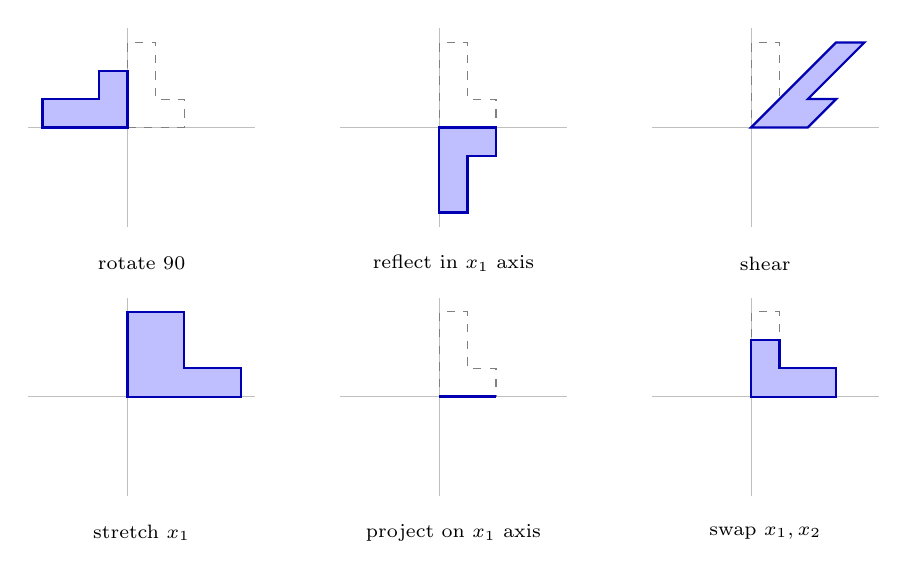
\begin{tikzpicture}[x=0.36cm,y=0.36cm,>=stealth,every node/.style={font=\scriptsize}]
  \foreach \cx/\cy in {0/0,11/0,22/0,0/-9.5,11/-9.5,22/-9.5}{
    \begin{scope}[shift={(\cx,\cy)}]
      \draw[gray!50] (-3.5,0)--(4.5,0); \draw[gray!50] (0,-3.5)--(0,3.5);
      \draw[dashed,gray] (0,0)--(2,0)--(2,1)--(1,1)--(1,3)--(0,3)--cycle;
    \end{scope}}
  \begin{scope}[shift={(0,0)}]
    \draw[thick,blue!70!black,fill=blue!25] (0,0)--(0,2)--(-1,2)--(-1,1)--(-3,1)--(-3,0)--cycle;
    \node at (0.5,-4.8) {rotate 90};
  \end{scope}
  \begin{scope}[shift={(11,0)}]
    \draw[thick,blue!70!black,fill=blue!25] (0,0)--(2,0)--(2,-1)--(1,-1)--(1,-3)--(0,-3)--cycle;
    \node at (0.5,-4.8) {reflect in $x_1$ axis};
  \end{scope}
  \begin{scope}[shift={(22,0)}]
    \draw[thick,blue!70!black,fill=blue!25] (0,0)--(2,0)--(3,1)--(2,1)--(4,3)--(3,3)--cycle;
    \node at (0.5,-4.8) {shear};
  \end{scope}
  \begin{scope}[shift={(0,-9.5)}]
    \draw[thick,blue!70!black,fill=blue!25] (0,0)--(4,0)--(4,1)--(2,1)--(2,3)--(0,3)--cycle;
    \node at (0.5,-4.8) {stretch $x_1$};
  \end{scope}
  \begin{scope}[shift={(11,-9.5)}]
    \draw[very thick,blue!70!black] (0,0)--(2,0);
    \node at (0.5,-4.8) {project on $x_1$ axis};
  \end{scope}
  \begin{scope}[shift={(22,-9.5)}]
    \draw[thick,blue!70!black,fill=blue!25] (0,0)--(0,2)--(1,2)--(1,1)--(3,1)--(3,0)--cycle;
    \node at (0.5,-4.8) {swap $x_1,x_2$};
  \end{scope}
\end{tikzpicture}
\end{center}

\textbf{Figure.} The L-shaped figure (dashed) and its image under six linear transformations of the plane, with matrices in the list below.

\begin{itemize}
  \item \textbf{Rotation by $90^\circ$}: $\begin{bmatrix}0&-1\\1&0\end{bmatrix}$. The vertex $(1,3)$ goes to $(-3,1)$.
  \item \textbf{Reflection in the $x_1$-axis}: $\begin{bmatrix}1&0\\0&-1\end{bmatrix}$, $(x_1,x_2)\mapsto(x_1,-x_2)$. The vertex $(1,3)$ goes to $(1,-3)$.
  \item \textbf{Horizontal shear}: $\begin{bmatrix}1&1\\0&1\end{bmatrix}$, $(x_1,x_2)\mapsto(x_1+x_2,x_2)$. The vertex $(1,3)$ goes to $(4,3)$; the $x_1$-axis does not move and each horizontal line slides right by its height.
  \item \textbf{Horizontal stretch by $2$}: $\begin{bmatrix}2&0\\0&1\end{bmatrix}$, $(x_1,x_2)\mapsto(2x_1,x_2)$. The vertex $(1,3)$ goes to $(2,3)$.
  \item \textbf{Projection onto the $x_1$-axis}: $\begin{bmatrix}1&0\\0&0\end{bmatrix}$, $(x_1,x_2)\mapsto(x_1,0)$. The whole figure is flattened onto the segment from $(0,0)$ to $(2,0)$.
  \item \textbf{Swap of the coordinates} (reflection in the line $x_2=x_1$): $\begin{bmatrix}0&1\\1&0\end{bmatrix}$, $(x_1,x_2)\mapsto(x_2,x_1)$. The vertex $(1,3)$ goes to $(3,1)$.
\end{itemize}

\begin{remark}
A reflection in the line through the origin that makes the angle $\alpha$ with the $x_1$-axis has the matrix $\begin{bmatrix}\cos2\alpha&\sin2\alpha\\\sin2\alpha&-\cos2\alpha\end{bmatrix}$. Indeed $\bv{e}_1$ lands on the unit vector at angle $2\alpha$ and $\bv{e}_2$ (at angle $90^\circ$) lands at angle $2\alpha-90^\circ$, which is $(\sin2\alpha,-\cos2\alpha)$. The choices $\alpha=0^\circ,45^\circ$ give the first and last reflections in the list.
\end{remark}

Notice what the pictures show: the rotation and the reflections keep the shape of the L (lengths and angles are preserved; the reflection reverses its orientation, a ``mirror image''); the shear and the stretch distort it but keep it a genuine two-dimensional figure; the projection collapses it. The next sections explain how to see these differences in the matrix.

\begin{exmp}{Do this, then that}{compose}
Let $\bv{y}=R_{90^\circ}\bv{x}$ and then $\bv{z}=F\bv{y}$, where $F=\begin{bmatrix}1&0\\0&-1\end{bmatrix}$ is the reflection in the $x_1$-axis. The composite $\bv{x}\mapsto\bv{z}$ is linear, because each step preserves sums and scalar multiples. Find its standard matrix, and then do the steps in the opposite order.

\textbf{Solution.} Follow the unit vectors. Rotate first: $\bv{e}_1\mapsto(0,1)\mapsto(0,-1)$ and $\bv{e}_2\mapsto(-1,0)\mapsto(-1,0)$. So the composite has standard matrix
\[
\begin{bmatrix}0&-1\\-1&0\end{bmatrix},
\]
the reflection in the line $x_2=-x_1$. Now reflect first and rotate afterward: $\bv{e}_1\mapsto(1,0)\mapsto(0,1)$ and $\bv{e}_2\mapsto(0,-1)\mapsto(1,0)$, giving
\[
\begin{bmatrix}0&1\\1&0\end{bmatrix},
\]
the swap of the coordinates, a reflection in the line $x_2=x_1$. The two results differ: \emph{order matters}.
\end{exmp}

\begin{think}{Does order matter?}{order}
(a)~In Example~\ref{ex:compose}, test the two composites on the point $(1,2)$ and see that they really are different transformations. (b)~Is there a pair of transformations from the catalogue for which the order does \emph{not} matter? (c)~Applying $R_{30^\circ}$ twice should be the same as applying $R_{60^\circ}$ once. Check this by following $\bv{e}_1$ through two steps, and explain which trigonometric identities this contains. (Section~2.1 will name the operation on matrices that this computes.)
\end{think}

\begin{kc}{Reading a picture}{reflect}
(a)~Write the standard matrix of the reflection in the $x_2$-axis, and the image of $(3,-2)$. (b)~What happens to a vector if you apply this reflection twice? What is the matrix of that composite?
\end{kc}

% ---------------------------------------------------------------------
\subsection*{One-to-one and onto}

Two questions about a function $T:\R^n\to\R^m$ come up constantly. Does every $\bv{b}$ in the codomain occur as an image? Can different inputs give the same output?

\begin{defn}{Onto and one-to-one}{ontoone}
A transformation $T:\R^n\to\R^m$ is \emph{onto} $\R^m$ if every $\bv{b}$ in $\R^m$ is the image of \emph{at least one} $\bv{x}$ in $\R^n$ (so the range is all of $\R^m$). It is \emph{one-to-one} if every $\bv{b}$ in $\R^m$ is the image of \emph{at most one} $\bv{x}$ in $\R^n$.
\end{defn}

For a linear map both properties can be read from the standard matrix. The pivot conditions are the ones you met in Sections 1.4 and 1.7; only the words are new.

\begin{thm}{Onto and one-to-one via pivots}{ontoone}
Let $T:\R^n\to\R^m$ be linear with standard matrix $A$ ($m\times n$).
\begin{enumerate}[label=(\alph*),itemsep=1pt]
  \item $T$ is \textbf{one-to-one} $\iff$ $T(\bv{x})=\bv{0}$ has only the trivial solution $\iff$ the columns of $A$ are linearly independent $\iff$ $A$ has a pivot in \emph{every column}.
  \item $T$ is \textbf{onto} $\R^m$ $\iff$ the columns of $A$ span $\R^m$ $\iff$ $A$ has a pivot in \emph{every row}.
\end{enumerate}
\end{thm}

\begin{proof}
(a)~If $T$ is one-to-one, then $T(\bv{x})=\bv{0}=T(\bv{0})$ forces $\bv{x}=\bv{0}$. Conversely, suppose $T(\bv{x})=\bv{0}$ only for $\bv{x}=\bv{0}$. If $T(\bv{x})=T(\bv{y})$, then $T(\bv{x}-\bv{y})=\bv{0}$ by Theorem~\ref{1.8-thm:sameimage}, so $\bv{x}-\bv{y}=\bv{0}$ and $\bv{x}=\bv{y}$. The remaining equivalences are Theorem~\ref{1.7-thm:cols}.
(b)~The range of $T$ is the span of the columns of $A$ (Definition~\ref{1.8-def:mattrans}); it is all of $\R^m$ exactly when $A\bv{x}=\bv{b}$ is solvable for every $\bv{b}$, which is Theorem~\ref{1.4-thm:existence}.
\end{proof}

Counting pivots gives quick consequences. A matrix with $m$ rows and $n$ columns has at most $\min(m,n)$ pivots. So if $n>m$ (more columns than rows), $T$ \emph{cannot} be one-to-one; if $m>n$, $T$ \emph{cannot} be onto; and if $m=n$, the two properties hold together or fail together.

\begin{center}
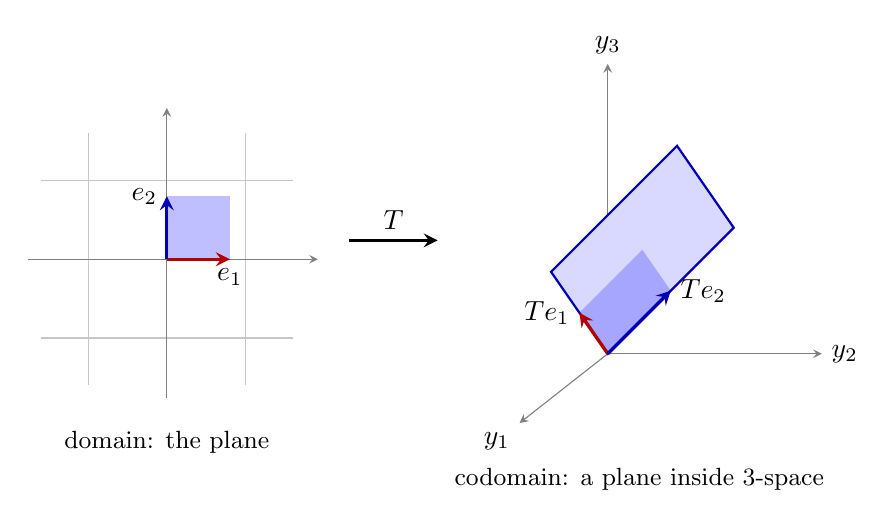
\begin{tikzpicture}[x=0.8cm,y=0.8cm,>=stealth]
  \draw[gray!45] (-2.0,-2.0) grid (2.0,2.0);
  \draw[->,gray] (-2.2,0)--(2.4,0); \draw[->,gray] (0,-2.2)--(0,2.4);
  \fill[blue!25] (0,0) rectangle (1,1);
  \draw[->,very thick,red!70!black] (0,0)--(1,0);
  \draw[->,very thick,blue!70!black] (0,0)--(0,1);
  \node[below] at (1,0) {$e_1$};
  \node[left] at (0,1) {$e_2$};
  \node at (0,-2.9) {\small domain: the plane};
  \draw[->,very thick] (2.9,0.3)--(4.3,0.3) node[midway,above] {$T$};
  \begin{scope}[shift={(7,-1.5)}]
    \draw[->,gray] (0,0)--(-1.4,-1.1); \node[below left] at (-1.4,-1.1) {$y_1$};
    \draw[->,gray] (0,0)--(3.4,0); \node[right] at (3.4,0) {$y_2$};
    \draw[->,gray] (0,0)--(0,4.6); \node[above] at (0,4.6) {$y_3$};
    \fill[blue!15] (0,0)--(-0.9,1.3)--(1.1,3.3)--(2,2)--cycle;
    \fill[blue!35] (0,0)--(-0.45,0.65)--(0.55,1.65)--(1,1)--cycle;
    \draw[thick,blue!70!black] (0,0)--(-0.9,1.3)--(1.1,3.3)--(2,2)--cycle;
    \draw[->,very thick,red!70!black] (0,0)--(-0.45,0.65);
    \draw[->,very thick,blue!70!black] (0,0)--(1,1);
    \node[left] at (-0.45,0.65) {$Te_1$};
    \node[right] at (1,1) {$Te_2$};
    \node at (0.5,-2.0) {\small codomain: a plane inside 3-space};
  \end{scope}
\end{tikzpicture}
\end{center}

\textbf{Figure.} The map $T(x_1,x_2)=(x_1,x_2,x_1+x_2)$ from $\R^2$ to $\R^3$ (Example~\ref{ex:ontoone}(i)). The unit square becomes the small parallelogram on $T(\bv{e}_1)=(1,0,1)$ and $T(\bv{e}_2)=(0,1,1)$, and the whole plane is laid onto the plane $y_3=y_1+y_2$ inside $\R^3$ (the larger parallelogram shows the image of the square $0\le x_1,x_2\le2$; $y_1,y_2,y_3$ are the coordinates in the codomain). Distinct inputs have distinct images, but the plane is a sheet inside $\R^3$ and leaves almost every point of $\R^3$ untouched.

\begin{exmp}{Three maps classified}{ontoone}
\textbf{(i)} $T(x_1,x_2)=(x_1,x_2,x_1+x_2)$ has the standard matrix $K=\begin{bmatrix}1&0\\0&1\\1&1\end{bmatrix}$ ($3\times2$). Two pivots, one in each column, so $T$ is \textbf{one-to-one}; but only two pivots for three rows, so $T$ is \textbf{not onto}. Its range is the plane $y_3=y_1+y_2$ (each column satisfies it, and the columns are independent).

\textbf{(ii)} $T(x_1,x_2,x_3)=(x_2-x_1,\ x_3-x_2)$ (the successive differences of a list of three numbers) has the standard matrix $D=\begin{bmatrix}-1&1&0\\0&-1&1\end{bmatrix}$ ($2\times3$). Row reducing:
\begin{align*}
\begin{bmatrix}-1&1&0\\0&-1&1\end{bmatrix}
&\rops{-R_1,\ -R_2}
\begin{bmatrix}1&-1&0\\0&1&-1\end{bmatrix}
\rops{R_1+R_2}
\begin{bmatrix}1&0&-1\\0&1&-1\end{bmatrix}.
\end{align*}
There is a pivot in each row, so $T$ is \textbf{onto} $\R^2$; column $3$ is free, so $T$ is \textbf{not one-to-one}. The vectors sent to $\bv{0}$ are the multiples of $(1,1,1)$: a constant list has no differences. By Theorem~\ref{1.8-thm:sameimage}, two lists with the same differences differ by a constant list.

\textbf{(iii)} Let $A(h)=\begin{bmatrix}1&-1&2\\0&1&1\\2&0&h\end{bmatrix}$ and $T(\bv{x})=A(h)\bv{x}$. Then
\begin{align*}
\begin{bmatrix}1&-1&2\\0&1&1\\2&0&h\end{bmatrix}
&\rops{R_3-2R_1}
\begin{bmatrix}1&-1&2\\0&1&1\\0&2&h-4\end{bmatrix}
\rops{R_3-2R_2}
\begin{bmatrix}1&-1&2\\0&1&1\\0&0&h-6\end{bmatrix}.
\end{align*}
If $h\neq6$ there are three pivots: $T$ is both one-to-one and onto. If $h=6$ there are only two pivots: $T$ is neither, since the third column is free (the null space is spanned by $(-3,-1,1)$; check: $A(6)(-3,-1,1)=(-3+1+2,\ -1+1,\ -6+6)=\bv{0}$) and the third row has no pivot (the range is a plane).
\end{exmp}

\begin{kc}{Classify}{classify}
Decide whether each linear map is one-to-one, onto, both or neither, using the standard matrix. (a)~$R_\theta$; \ (b)~the projection onto the $x_1$-axis; \ (c)~the shear $\begin{bmatrix}1&1\\0&1\end{bmatrix}$; \ (d)~$\begin{bmatrix}1&0\\0&1\\2&3\end{bmatrix}$; \ (e)~$\begin{bmatrix}1&2&0\\0&1&1\end{bmatrix}$; \ (f)~$\begin{bmatrix}1&2\\2&4\end{bmatrix}$.
\end{kc}

\begin{think}{Dimension counting}{dimcount}
(a)~Why can a linear map $\R^3\to\R^2$ never be one-to-one? Give an argument with pivots, and a geometric one (what must happen to some line?). (b)~Why can a linear map $\R^2\to\R^3$ never be onto? (c)~Can a linear map $\R^2\to\R^2$ be one-to-one but not onto? Explain.
\end{think}

\begin{think}{Flattening and area}{area}
The unit square has area $1$. Compute the area of its image under each of the following: the shear, the rotation by $90^\circ$, the stretch by $2$, the projection onto the $x_1$-axis, the reflection in the $x_1$-axis, and $M=\begin{bmatrix}2&1\\-1&1\end{bmatrix}$ of Section~1.8. (The image is the parallelogram on the two columns; its area is $|ad-bc|$ for the matrix $\begin{bmatrix}a&b\\c&d\end{bmatrix}$, but consider the signed value $ad-bc$ too.) Which maps are one-to-one? What do you notice about the area of the image and one-to-one? What does the \emph{sign} of $ad-bc$ say about the reflection?
\end{think}

\begin{think}{Undoing a map}{undo}
A map that is both one-to-one and onto sends each $\bv{b}$ to exactly one $\bv{x}$, so it can be undone. What undoes $R_\theta$? What undoes the shear $\begin{bmatrix}1&1\\0&1\end{bmatrix}$? What would it mean to undo the projection onto the $x_1$-axis?
\end{think}

\subsection*{Summary}
\begin{itemize}
  \item Every linear transformation $T:\R^n\to\R^m$ is a matrix transformation $T(\bv{x})=A\bv{x}$, with the unique \textbf{standard matrix} $A=[\,T(\bv{e}_1)\ \cdots\ T(\bv{e}_n)\,]$: the $j$th column is the image of $\bv{e}_j$.
  \item To find $A$: substitute the unit vectors into a formula, read the images of $\bv{e}_1,\bv{e}_2$ from a picture, or express $\bv{e}_j$ through given vectors and use superposition.
  \item \textbf{Geometry of the plane:} the rotation by $\theta$ is $\begin{bmatrix}\cos\theta&-\sin\theta\\\sin\theta&\cos\theta\end{bmatrix}$; reflections, shears, stretches and projections have simple matrices (the catalogue). The columns tell where the grid goes.
  \item A composite of linear maps is linear; its matrix is found by following $\bv{e}_1,\dots,\bv{e}_n$ through the steps. \textbf{Order matters.}
  \item $T$ is \textbf{one-to-one} iff $A$ has a pivot in every column (independent columns, only $\bv{0}\mapsto\bv{0}$); $T$ is \textbf{onto} iff $A$ has a pivot in every row (columns span $\R^m$).
  \item $n>m$ forbids one-to-one; $m>n$ forbids onto; for square matrices the two properties go together. A projection flattens the plane and is neither.
\end{itemize}

\subsection*{Questions to think about before the next section}
\begin{enumerate}
  \item You applied two linear maps in a row in Example~\ref{ex:compose}. Can you describe the matrix of the composite directly in terms of the two matrices? Try it for the rotation by $90^\circ$ followed by the shear $\begin{bmatrix}1&2\\0&1\end{bmatrix}$.
  \item If $T$ is a one-to-one and onto linear map with matrix $A$, what should the matrix of the map that undoes $T$ be? Find it for the shear $\begin{bmatrix}1&1\\0&1\end{bmatrix}$.
  \item For a square matrix, one-to-one and onto go together. Which of the earlier characterisations of ``every column is a pivot column'' and ``every row is a pivot row'' have you now seen to coincide?
\end{enumerate}

\subsection*{Answers and discussion}
\begin{description}[leftmargin=0pt,itemsep=5pt]
  \item[Knowledge Check \ref{kc:matdata}.] (a)~$A=\begin{bmatrix}2&0\\-1&3\end{bmatrix}$; $T(3,-2)=3(2,-1)-2(0,3)=(6,-9)$. Check by rows: $2\cdot3+0\cdot(-2)=6$ and $-1\cdot3+3\cdot(-2)=-9$. (b)~$T(\bv{e}_1)=(1,0)$, $T(\bv{e}_2)=(0,1)$, $T(\bv{e}_3)=(0,-1)$, $T(\bv{e}_4)=(4,0)$, so $A=\begin{bmatrix}1&0&0&4\\0&1&-1&0\end{bmatrix}$, a $2\times4$ matrix (domain $\R^4$, codomain $\R^2$).
  \item[Knowledge Check \ref{kc:rot}.] (a)~$R_{180^\circ}=\begin{bmatrix}-1&0\\0&-1\end{bmatrix}$ sends $(2,3)$ to $(-2,-3)$; $R_{-90^\circ}=\begin{bmatrix}0&1\\-1&0\end{bmatrix}$ sends $(2,3)$ to $(3,-2)$, a quarter-turn to the right. (b)~$R_{60^\circ}=\begin{bmatrix}\tfrac12&-\tfrac{\sqrt3}{2}\\\tfrac{\sqrt3}{2}&\tfrac12\end{bmatrix}$; $R_{60^\circ}(2,0)=(1,\sqrt3)$. (c)~Yes, one-to-one (indeed the columns are independent: they are perpendicular unit vectors), and yes, a line through the origin goes to a line through the origin (Theorem~\ref{1.8-thm:lines}, with direction rotated).
  \item[Knowledge Check \ref{kc:reflect}.] (a)~$\begin{bmatrix}-1&0\\0&1\end{bmatrix}$; $(3,-2)\mapsto(-3,-2)$. (b)~Applying it twice returns every vector to itself, so the composite is the identity matrix $\begin{bmatrix}1&0\\0&1\end{bmatrix}$: a reflection undoes itself.
  \item[Knowledge Check \ref{kc:classify}.] (a)~Both: the $2\times2$ matrix has two pivots. (b)~Neither: pivot only in the first row and first column. (c)~Both: the matrix is upper triangular with two pivots. (d)~One-to-one (two pivots, one per column) but not onto ($3$ rows, $2$ pivots). (e)~Onto (a pivot in each row) but not one-to-one (column $3$ is free). (f)~Neither: the second column is twice the first, so there is only one pivot.
  \item[Pause and think \ref{think:whyunit}.] (a)~No. If $A\bv{x}=B\bv{x}$ for all $\bv{x}$, take $\bv{x}=\bv{e}_j$: the $j$th columns agree, so $A=B$. (b)~The vectors $\bv{v}_1,\dots,\bv{v}_n$ must span $\R^n$ (equivalently, since there are $n$ of them, be independent). Then each $\bv{e}_j$ is a combination of them, with weights found by row reduction as in Example~\ref{1.8-ex:values}, and superposition gives $T(\bv{e}_j)$. If they do not span, some $\bv{e}_j$ is not reachable and the standard matrix is not determined.
  \item[Pause and think \ref{think:order}.] (a)~$(1,2)$: rotate then reflect: $R_{90^\circ}(1,2)=(-2,1)\mapsto(-2,-1)$; reflect then rotate: $F(1,2)=(1,-2)\mapsto R_{90^\circ}(1,-2)=(2,1)$. Different points. (b)~Yes. Two rotations commute: $R_\varphi R_\theta=R_\theta R_\varphi=R_{\varphi+\theta}$; the reflection in the $x_1$-axis and the reflection in the $x_2$-axis commute (both composites are $R_{180^\circ}$); and any map composed with the identity. In general, though, order matters. (c)~$R_{30^\circ}\bv{e}_1=(\tfrac{\sqrt3}{2},\tfrac12)$. Apply $R_{30^\circ}$ again: $\bigl(\tfrac{\sqrt3}{2}\cdot\tfrac{\sqrt3}{2}-\tfrac12\cdot\tfrac12,\ \tfrac12\cdot\tfrac{\sqrt3}{2}+\tfrac{\sqrt3}{2}\cdot\tfrac12\bigr)=(\tfrac12,\tfrac{\sqrt3}{2})$, the first column of $R_{60^\circ}$. In general the first column of $R_\varphi R_\theta$ is $(\cos\varphi\cos\theta-\sin\varphi\sin\theta,\ \sin\varphi\cos\theta+\cos\varphi\sin\theta)$ and it equals $(\cos(\varphi+\theta),\sin(\varphi+\theta))$: these are the angle-addition formulas.
  \item[Pause and think \ref{think:dimcount}.] (a)~A $2\times3$ matrix has at most $2$ pivots but $3$ columns, so some column is free: $A\bv{x}=\bv{0}$ has a nonzero solution, that is, a nonzero vector is sent to $\bv{0}$ just as $\bv{0}$ is. Geometrically a line of inputs is collapsed to a point (Example~\ref{ex:ontoone}(ii)). (b)~A $3\times2$ matrix has at most $2$ pivots but $3$ rows, so some row has no pivot, and the range, a span of two vectors, is at most a plane inside $\R^3$ (Figure of Example~\ref{ex:ontoone}(i)). (c)~No. For a $2\times2$ matrix, pivot in every column means two pivots, which is a pivot in each of the two rows; so one-to-one implies onto, and conversely.
  \item[Pause and think \ref{think:area}.] Shear: columns $(1,0),(1,1)$, signed area $1\cdot1-1\cdot0=1$. Rotation by $90^\circ$: $0\cdot0-(-1)\cdot1=1$. Stretch: $2\cdot1-0=2$. Projection: $1\cdot0-0\cdot0=0$: the image is a segment, with zero area. Reflection: $1\cdot(-1)-0=-1$, area $1$ in absolute value. $M$: $2\cdot1-1\cdot(-1)=3$. The maps with nonzero area (shear, rotation, stretch, reflection, $M$) are one-to-one; the projection has area $0$ and is not one-to-one. This suggests ``one-to-one iff $ad-bc\neq0$'', which is true and is the determinant of Chapter 3. The sign records whether the map reverses orientation: the reflection turns a counterclockwise pair of axes into a clockwise one, which is why the L comes out as its mirror image.
  \item[Pause and think \ref{think:undo}.] $R_\theta$ is undone by the rotation by $-\theta$, $R_{-\theta}$. The shear $(x_1,x_2)\mapsto(x_1+x_2,x_2)$ is undone by sliding back, $(y_1,y_2)\mapsto(y_1-y_2,y_2)$, with the matrix $\begin{bmatrix}1&-1\\0&1\end{bmatrix}$. The projection cannot be undone: all the points $(x_1,x_2)$ with the same $x_1$ land on one point, and from that point you cannot tell which one you started from (the map is not one-to-one); and points off the axis are never reached (not onto).
  \item[Before the next section.] (1)~Rotate then shear: $\bv{e}_1\mapsto(0,1)\mapsto(2,1)$ and $\bv{e}_2\mapsto(-1,0)\mapsto(-1,0)$, so the composite has matrix $\begin{bmatrix}2&-1\\1&0\end{bmatrix}$. The columns are the shear matrix applied to the columns of the rotation matrix: that is how Section~2.1 will define the product. (2)~The map that slides back: $\begin{bmatrix}1&-1\\0&1\end{bmatrix}$. (3)~Both conditions say the same thing for a square matrix, as in Pause and think~\ref{think:dimcount}(c): independent columns and spanning columns coincide.
\end{description}

\end{document}
